\documentclass[t]{beamer}
\usepackage[T1]{fontenc}
\usepackage[utf8]{inputenc}
\usepackage{lmodern}
\usepackage{lmodern}
\usepackage{biblatex} 
\usepackage{amsmath}
\usepackage{amsfonts}
\usepackage{amssymb}
\usepackage{amsthm}
\usepackage{graphicx}
\usepackage{color}
\usepackage{xcolor}
\usepackage{url}
\usepackage{textcomp}
\usepackage{hyperref}
\usepackage{parskip}
\usepackage{svg}
\usepackage{caption}

\usetheme{CambridgeUS}
\AtBeginBibliography{\footnotesize}
\addbibresource{presentation.bib}

\makeatletter
\setbeamertemplate{footline}
{
  \leavevmode%
  \hbox{%
  \begin{beamercolorbox}[wd=.333333\paperwidth,ht=2.25ex,dp=1ex,center]{author in head/foot}%
    \usebeamerfont{author in head/foot}\insertshortauthor%~~\beamer@ifempty{\insertshortinstitute}{}{(\insertshortinstitute)}
  \end{beamercolorbox}%
  \begin{beamercolorbox}[wd=.333333\paperwidth,ht=2.25ex,dp=1ex,center]{title in head/foot}%
    \usebeamerfont{title in head/foot}\insertshorttitle
  \end{beamercolorbox}%
  \begin{beamercolorbox}[wd=.333333\paperwidth,ht=2.25ex,dp=1ex,right]{date in head/foot}%
    \usebeamerfont{date in head/foot}\insertshortdate{}\hspace*{2em}
    \insertframenumber{} / \inserttotalframenumber\hspace*{2ex} 
  \end{beamercolorbox}}%
  \vskip0pt%
}
\makeatother

\title{Knowledge-Based Question Answering}
\author{Sudipto Ghosh}
\institute{\emph{M.Sc. CS Semester I\\Department of Computer Science\\University of Delhi}}
\date{\today}

\begin{document}

\begin{frame}
    \titlepage
\end{frame}

\section{Model Training}
\begin{frame}
    \frametitle{Model Training}

    \begin{itemize}
        \item data preparation and kb population -- sc judgements from 1970-2010 (source: indiankanoon.org)
        \item metadata extraction using jape grammar rules
        \item fine-tuned gpt with two-way prompt-completion pairs
    \end{itemize}
\end{frame}

\section{Basic Prototype}
\begin{frame}
    \frametitle{Basic Prototype}

    \centering 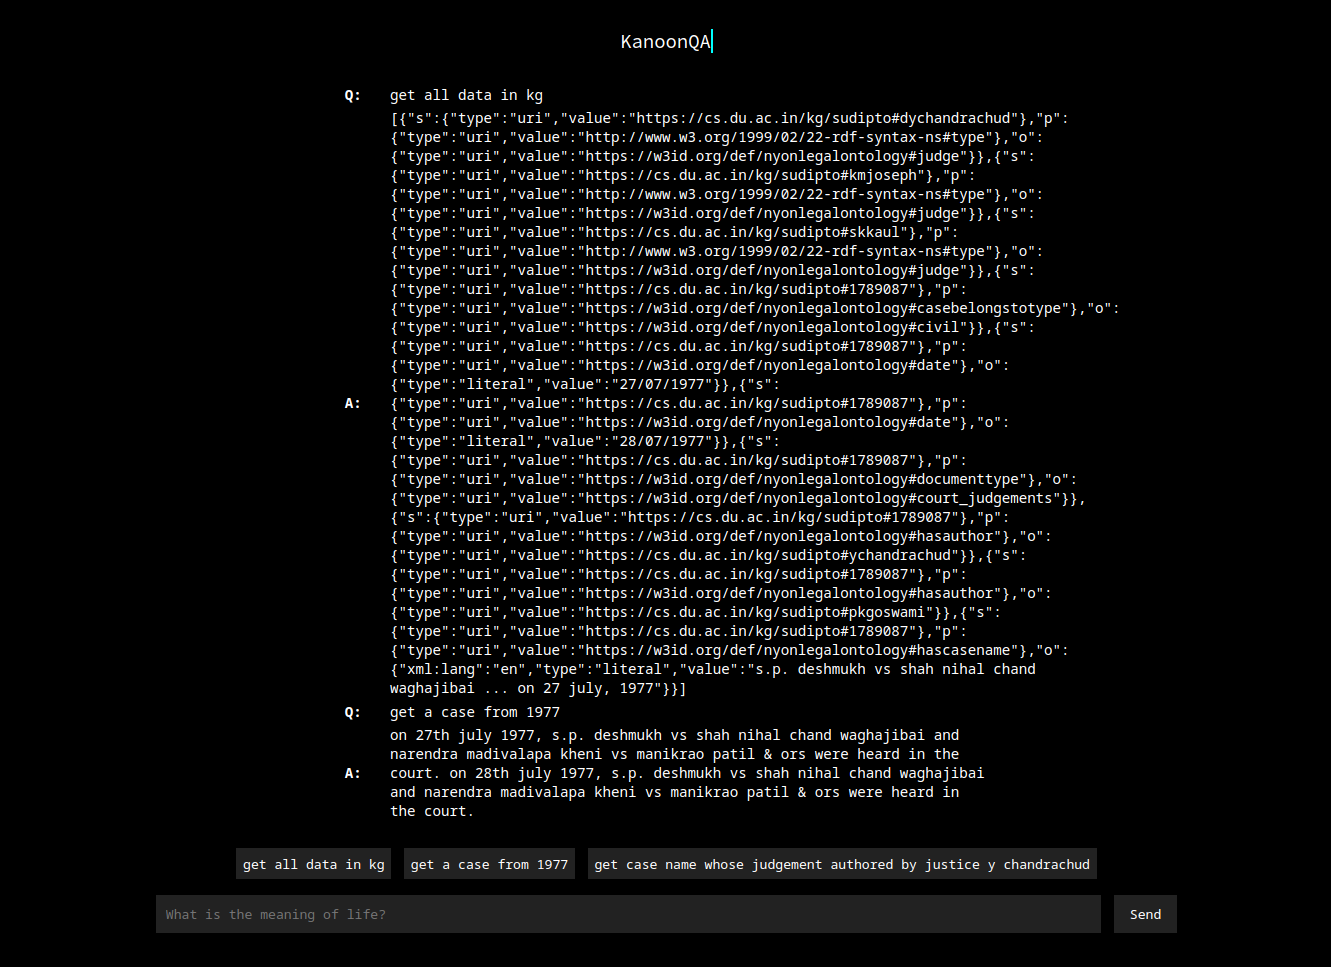
\includegraphics[width=270pt]{./Screenshot from 2023-03-03 09-18-51.png}\\
   \tiny{user interface and output\\tech stack: next.js, google cloud platform}
\end{frame}

\section{Basic Prototype}
\begin{frame}
    \frametitle{Basic Prototype}

    \centering 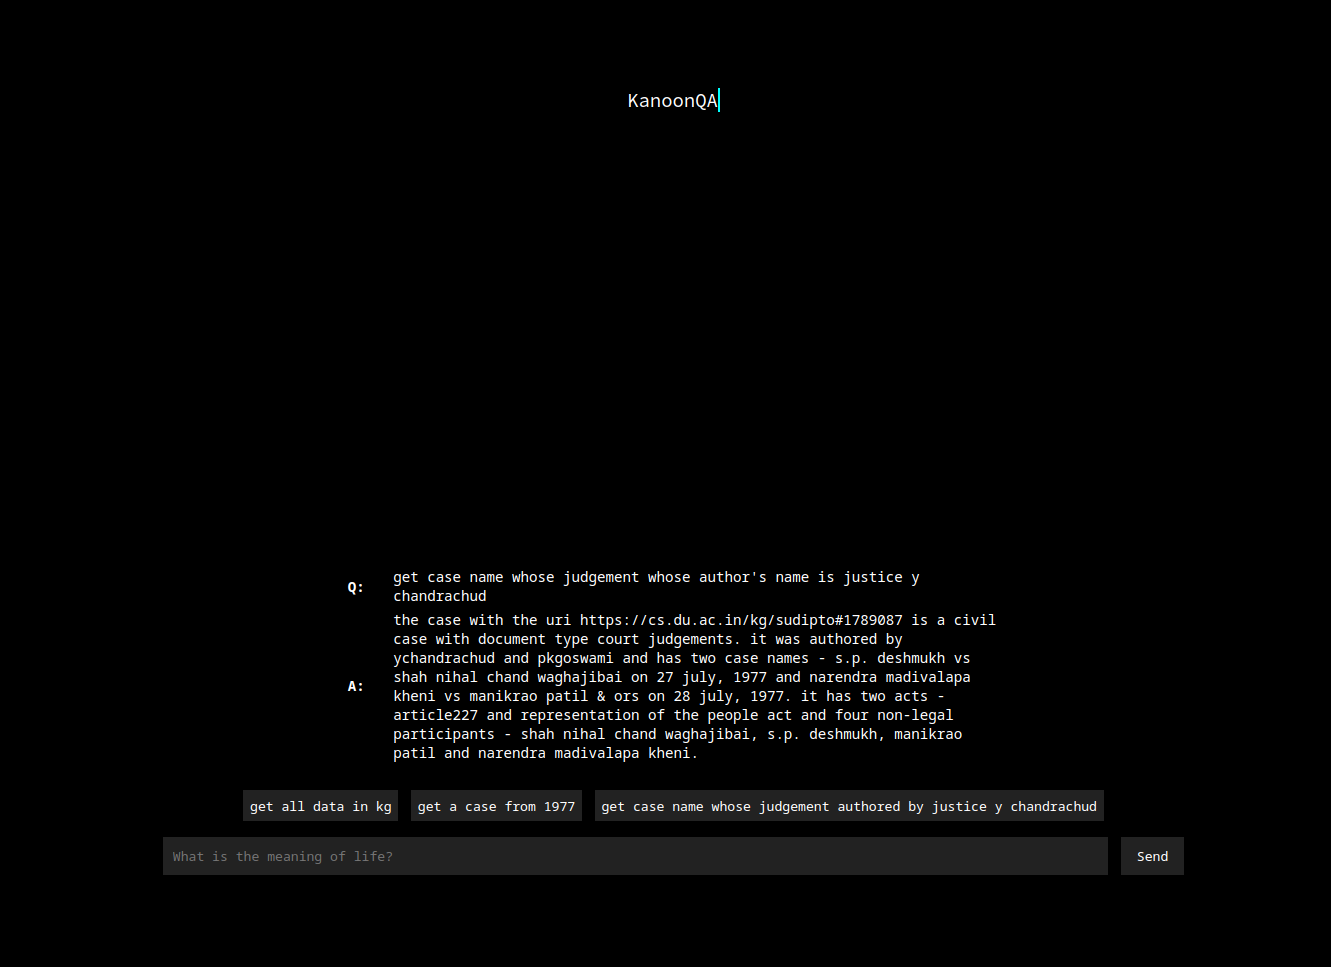
\includegraphics[width=270pt]{./Screenshot from 2023-03-03 09-34-53.png}\\
   \tiny{user interface and output\\tech stack: next.js, google cloud platform}
\end{frame}

\section{Competency Questions}
\begin{frame}
    \frametitle{Competency Questions}

    \begin{itemize}
        \item get all data in kg
        \item get cases from 1977
        \item get a case whose judgement was authored by justice y chandrachud
        \item list all civil cases
    \end{itemize}
\end{frame}

\end{document}